\section{Dinamica Manipolatore}
Il modello dinamico del manipolatore ci fornisce una descrizione matematica della relazione che è instaurata tra le forze agenti sul robot (generalizzate) ed il movimento prodotto dalla sua struttura, cioè le configurazioni che assume nel tempo. Inizialmente, nel calcolo della dinamica sono stati usati tre metodi diversi, il metodo delle azioni vincolari, il metodo di Lagrange e quello dei lavori virtuali. Si è poi deciso di proseguire esclusivamente con il PLV. L'obiettivo di questa sezione è quello di mostrare l'approccio e i risultati ottenuti per il calcolo della dinamica diretta ed inversa.
\subsection{Prerequisiti per il calcolo della dinamica}\label{sec:prerequisiti-dinamica}
Prima di andare ad analizzare i metodi utilizzati, è importante andare a ricavare tutte le matrici delle quali avremo bisogno, in particolare è necessario andare a definire delle matrici che ci permettano di ottenere $\theta_3$ e $\theta_4$ in funzione di $\theta_1$ e $\theta_2$.
\subsubsection{Jacobiana $J_{34}$ e calcolo $\dot{\theta_3},\dot{\theta_4}$}
A partire da $\theta_1, \theta_2$ possiamo, mediante la cinematica diretta ottenere $\theta_3$ e $\theta_4$. Dall'equazione dei loop vettoriali \ref{eq:loopVettoriali} derivandola otteniamo: 
\begin{equation}
	\begin{cases}
		-\sin\theta_1 \dot{\theta_1} -\sin\theta_3\dot{\theta_3}+\sin\theta_2\dot{\theta_2}+\sin\theta_4\dot{\theta_4} = 0
		\\ \cos\theta_1\dot{\theta_1} + \cos\theta_3\dot{\theta_3}-\cos\theta_2\dot{\theta_2}-\cos\theta_4\dot{\theta_4} = 0
	\end{cases}
\end{equation}
Considerando anche le velocità $\dot{\theta_1}$ e $\dot{\theta_2}$ possiamo dobbiamo ricavare $\dot{\theta_3}, \dot{\theta_4}$, per far questo dalla seconda equazione ricaviamo $\dot{\theta_4}$ in funzione di $\dot{\theta_3}$:
\begin{equation*}
	\dot{\theta_4} = \frac{\cos\theta_1\dot{\theta_1} + \cos\theta_3\dot{\theta_3}-\cos\theta_2\dot{\theta_2}}{\cos\theta_4}
\end{equation*}
Sostituendo $\dot{\theta_4}$ nella prima equazione otteniamo:
\begin{equation*}
	\cos\theta_4(-\sin\theta_1\dot{\theta_1}-\sin\theta_3\dot{\theta_3}+\sin\theta_2\dot{\theta_2})+\tan\theta_4(\cos\theta_1\dot{\theta_1}+\cos\theta_3\dot{\theta_3}-\cos\theta_2\dot{\theta_2}) = 0
\end{equation*}
Da questa possiamo ricavare $\dot{\theta_3}$ come:
\begin{equation}
	\dot{\theta_3} = \frac{N_{13}}{D_{13}}\dot{\theta_1}+\frac{N_{23}}{D_{13}}\dot{\theta_2}
\end{equation}
dove:
\begin{equation*}
    N_{13} = \frac{\cos\theta_4}{\sin\theta_4}\sin\theta_1-\cos\theta_1
\end{equation*}
\begin{equation*}
    N_{23} = \cos\theta_2-\frac{\cos\theta_4}{\sin\theta_4}\sin\theta_2
\end{equation*}
\begin{equation*}
    D_{13} = \cos\theta_3-\frac{\cos\theta_4}{\sin\theta_4}\sin\theta_3
\end{equation*}
Avendo ottenuto questo valore possiamo anche esprimere $\dot{\theta_4}$ come:
\begin{equation}
	\dot{\theta_4} = \frac{N_{14}}{D_{14}}\dot{\theta_1}+\frac{N_{24}}{D_{14}}\dot{\theta_2}
\end{equation} 
dove:
\begin{equation*}
    N_{14} = \frac{\sin\theta_1\cos\theta_3}{\sin\theta_3}-\frac{\cos\theta_4}{\sin\theta_4}+\frac{\cos\theta_4}{\sin\theta_4}\sin\theta_1 - \cos\theta_1
\end{equation*}
\begin{equation*}
    N_{24} = -\frac{\sin\theta_2\cos\theta_3}{\sin\theta_3}-\frac{\cos\theta_4}{\sin\theta_4}-\frac{\cos\theta_4}{\sin\theta_4}\sin\theta_2+\cos\theta_2
\end{equation*}
\begin{equation*}
    D_{14} = \frac{\sin\theta_4\cos\theta_3}{\sin\theta_3}-\frac{\cos\theta_4}{\sin\theta_4}
\end{equation*}
Il passo finale è quello di andare a rappresentare la matrice jacobiana che lega le velocità $\dot{\theta_3}$ e $\dot{\theta_4}$ con le velocità in ingresso al manipolatore:
\begin{equation}
    J_{34} = \begin{bmatrix}
    \frac{N_{13}}{D_{13}} & \frac{N_{23}}{D_{13}} \\
    \frac{N_{14}}{D_{14}} & \frac{N_{24}}{D_{14}}
    \end{bmatrix}
\end{equation}
%Notiamo che possiamo esprimere i parametri appena calcolati anche come:
%\begin{equation*}
%	\begin{bmatrix}
%		\dot{\theta_3} \\ \dot{\theta_4}
%	\end{bmatrix} = J_{34}\begin{bmatrix}
%	\dot{\theta_1} \\ \dot{\theta_2}
%\end{bmatrix}
%\end{equation*}
\subsubsection{Jacobiana $\dot{J_{34}}$ e calcolo di $\ddot{\theta_3}, \ddot{\theta_4}$}
Per andar ad ottenere la jacobiana finale, ed i valori delle accelerazioni sui giunti non motorizzati occorre derivare tutti gli elementi visti in precedenza, in particolare:
\begin{equation*} %  N11p =  N13p
    \dot{N_{13}} = \frac{-1}{\sin^2\theta_4\cdot\dot{\theta_4}\sin\theta_1}+\frac{\cos\theta_4}{\sin\theta_4}\cos\theta_1\dot{\theta_1}+\sin\theta_1\dot{\theta_1}
\end{equation*}
\begin{equation*} %N12p = N23p
   \dot{N_{23}} =\frac{1}{\sin^2\theta_4\cdot\dot{\theta_4}\sin\theta_2}-\frac{\cos\theta_4}{\sin\theta_4}\cos\theta_2\dot{\theta_2}-\sin\theta_2\dot{\theta_2}
\end{equation*}
\begin{equation*} % D1p = D13p
  \dot{D_{13}} =  -\sin\theta_3\dot{\theta_3} + \frac{1}{\sin^2\theta_4}\dot{\theta_4}\sin\theta_3 -\frac{ \cos\theta_4} {\sin\theta_4}\cos\theta_3\dot{\theta_3}
\end{equation*}
\begin{equation*} % N21p = N14p
\begin{aligned}
    \dot{N_{14}} = \cos\theta_1\dot{\theta_1}\bigg(\frac{\cos\theta_3}{\sin\theta_3}-\frac{\cos\theta_4}{\sin\theta_4}\bigg) + \sin\theta_1\bigg(\frac{1}{\sin^2\theta_3}\dot{\theta_3}+\frac{1}{\sin^2\theta_4}\dot{\theta_4}\bigg)+\\+\frac{-1}{\sin^2\theta_4}\dot{\theta_4}\sin\theta_1 +\cot\theta_4\cos\theta_1\dot{\theta_1}+\sin\theta_1\dot{\theta_1}
    \end{aligned}
\end{equation*}
\begin{equation*} % N22p = N24p
    \begin{aligned}
    \dot{N_{24}} = -\cos\theta_2\dot{\theta_2}\bigg(\frac{\cos\theta_3}{\sin\theta_3} - \frac{\cos\theta_4}{\sin\theta_4} \bigg) - \sin\theta_2\bigg(\frac{-1}{\sin^2\theta_3}\dot{\theta_3} + \frac{1}{\sin^2\theta_4}\dot{\theta_4}\bigg) -\\
    - \frac{-1}{\sin^2\theta_4}\dot{\theta_4}\sin\theta_2-\cot\theta_4\cos\theta_2\dot{\theta_2}-\sin\theta_2\dot{\theta_2}
    \end{aligned}
\end{equation*}
\begin{equation*} % D2p = D14p
   \dot{D_{14}} = \cos\theta_4\dot{\theta_4}(\cot\theta_3-\cot\theta_4)+\sin\theta_4\bigg(\frac{-1}{\sin^2\theta_3}\dot{\theta_3} + \frac{1}{\sin^2\theta_4}\dot{\theta_4}\bigg)
\end{equation*}
Esprimendo la matrice jacobiana $\dot{J_{34}}$ in funzione dei parametri appena trovati scriviamo:
\begin{equation}
    \dot{J_{34}} =
    \begin{bmatrix}
    \frac{\dot{N_{13}}D_{13}-N_{13}\dot{D_{13}}}{D_{13}^2} & 
     \frac{\dot{N_{23}}D_{13}-N_{23}\dot{D_{13}}}{D_{13}^2} \\
    \frac{\dot{N_{14}}D_{14}-N_{14}\dot{D_{14}}}{D_{14}^2} &
     \frac{\dot{N_{24}}D_{14}-N_{24}\dot{D_{14}}}{D_{14}^2}
    \end{bmatrix}
\end{equation}
Per concludere andiamo a trovare:
\begin{equation}
    \begin{bmatrix}
    \ddot{\theta_3} \\ \ddot{\theta_4}
    \end{bmatrix}
    = 
    \dot{J_{34}}\begin{bmatrix}
    \dot{\theta_1} \\ \dot{\theta_2}
    \end{bmatrix} + 
    J_{34} \begin{bmatrix}
    \ddot{\theta_1} \\ \ddot{\theta_2}
    \end{bmatrix}
\end{equation}
\subsubsection{Matrici di inerzia}
Per trovare la soluzione all'equazione del PLV introduciamo le matrici che hanno avuto un ruolo fondamentale nel calcolo:
\begin{equation*}
    J_1 = \begin{bmatrix}
     -0.5l\sin\theta_1 & 0 \\ 0.5l\cos\theta_1 & 0
    \end{bmatrix} \Rightarrow
    \dot{J_1} = \begin{bmatrix}
     -0.5l\cos\theta_1\dot{\theta_1} & 0 \\ -0.5l\sin\theta_1\dot{\theta_1} & 0
    \end{bmatrix}
\end{equation*}
\begin{equation*}
    J_2 = \begin{bmatrix}
           0 & -0.5l\sin\theta_2 \\
           0 & 0.5l\cos\theta_2 
           \end{bmatrix}
           \Rightarrow
   \dot{J_2} = \begin{bmatrix} 0 & -0.5l\cos\theta_2\dot{\theta_2} \\
           0 & -0.5l\sin\theta_2\dot{\theta_2}
           \end{bmatrix}
\end{equation*}
\begin{equation*}
    J_3 = \begin{bmatrix}
    -l\sin\theta_1+0.5\sin\theta_3 \frac{N_{13}}{D_{13}} & 
    -0.5l\sin\theta_3 \frac{N_{23}}{D_{13}} \\
    l\cos\theta_1+0.5\cos\theta_3 \frac{N_{13}}{D_{13}} & 
    0.5l\cos\theta_3 \frac{N_{13}}{D_{23}}
    \end{bmatrix}
\end{equation*}
\begin{equation*}
    J_4 = \begin{bmatrix}
    -0.5l\sin\theta_4 \frac{N_{14}}{D_{14}} &
    -l\sin\theta_2+0.5\sin\theta_4\frac{N_{24}}{D_{14}} \\
    0.5l\cos\theta_4\frac{N_{14}}{D_{14}} &
    l\cos\theta_2+0.5\cos\theta_4 \frac{N_{24}}{D_{14}}
    \end{bmatrix}
\end{equation*}
In particolare, le matrici assumo il significato di jacobiano che consente il passaggio dalle coordinate dei giunti alle coordinate baricentriche dei quattro link. 
\begin{equation*}
	\begin{bmatrix}
		\dot{x}_{g1} \\ \dot{y}_{g1}
	\end{bmatrix} = J_1 \begin{bmatrix}
	\dot{\theta_1} \\ \dot{\theta_2}
\end{bmatrix} , \ \ 
	\begin{bmatrix}
	\ddot{x}_{g1} \\ \ddot{y}_{g1}
\end{bmatrix} = J_1 \begin{bmatrix}
	\ddot{\theta_1} \\ \ddot{\theta_2}
\end{bmatrix} + \dot{J_1} \begin{bmatrix}
\dot{\theta_1} \\ \dot{\theta_2}
\end{bmatrix}
\end{equation*}
\begin{equation*}
	\begin{bmatrix}
		\dot{x}_{g2} \\ \dot{y}_{g2}
	\end{bmatrix} = J_2 \begin{bmatrix}
		\dot{\theta_1} \\ \dot{\theta_2}
	\end{bmatrix} , \ \ 
	\begin{bmatrix}
		\ddot{x}_{g2} \\ \ddot{y}_{g2}
	\end{bmatrix} = J_2 \begin{bmatrix}
		\ddot{\theta_1} \\ \ddot{\theta_2}
	\end{bmatrix} + \dot{J_2} \begin{bmatrix}
		\dot{\theta_1} \\ \dot{\theta_2}
	\end{bmatrix}
\end{equation*}
\begin{equation*}
	\begin{bmatrix}
		\dot{x}_{g3} \\ \dot{y}_{g3}
	\end{bmatrix} = J_3 \begin{bmatrix}
		\dot{\theta_1} \\ \dot{\theta_2}
	\end{bmatrix} , \ \ 
	\begin{bmatrix}
		\ddot{x}_{g3} \\ \ddot{y}_{g3}
	\end{bmatrix} = J_3 \begin{bmatrix}
		\ddot{\theta_1} \\ \ddot{\theta_2}
	\end{bmatrix} + \dot{J_3} \begin{bmatrix}
		\dot{\theta_1} \\ \dot{\theta_2}
	\end{bmatrix}
\end{equation*}
\begin{equation*}
	\begin{bmatrix}
		\dot{x}_{g4} \\ \dot{y}_{g4}
	\end{bmatrix} = J_4 \begin{bmatrix}
		\dot{\theta_1} \\ \dot{\theta_2}
	\end{bmatrix} , \ \ 
	\begin{bmatrix}
		\ddot{x}_{g4} \\ \ddot{y}_{g4}
	\end{bmatrix} = J_4 \begin{bmatrix}
		\ddot{\theta_1} \\ \ddot{\theta_2}
	\end{bmatrix} + \dot{J_4} \begin{bmatrix}
		\dot{\theta_1} \\ \dot{\theta_2}
	\end{bmatrix}
\end{equation*}
Importanti nel calcolo della dinamica sono anche le derivate delle matrici che abbiamo appena visto, ovvero $\dot{J_3}, \dot{J_4}$,  riportate in appendice \ref{appendice:t34punto}
\subsection{Principio dei lavori virtuali}
Il lavoro virtuale è il lavoro svolto da una forza reale che agisce attraverso uno spostamento virtuale o da una forza virtuale che agisce attraverso uno spostamento reale.
Uno spostamento virtuale è uno spostamento coerente con i vincoli della struttura, cioè che soddisfano le condizioni al contorno in corrispondenza degli appoggi.
Una forza virtuale è un qualsiasi sistema di forze in equilibrio.
Per problemi nei quali i corpo sono composti da membri interconnessi che si possono muovere relativamente gli uni rispetto agli altri, originando diverse configurazioni di equilibrio un buon metodo di analisi è quello del "principio dei lavori virtuali" conosciuto anche come PLV ci permette di ottenere una relazione relativamente semplice, è basato sul concetto di Lavoro sviluppato da una forza, ed inoltre ci consente di analizzare la stabilità di un sistema in equilibrio.
\begin{equation}
    \sum_{i=1}^m F_j\delta q_j\label{eq:din}
\end{equation}
\subsection{Dinamica inversa}
Il problema della dinamica inversa consiste nel determinare le coppie ai giunti necessarie per generare il movimento a partire da posizione, velocità ed accelerazione.
\\Andando a sviluppare l'equazione dei principi virtuali troviamo le coppie dei link motorizzati nel seguente modo:
\begin{equation}
\begin{split}
\begin{bmatrix}
\delta \theta_1 & \delta \theta_2
\end{bmatrix}
\begin{bmatrix}
C_1 \\ C_2
\end{bmatrix} 
= \begin{bmatrix}
\delta \theta_1 & \delta \theta_2
\end{bmatrix} J_r \begin{bmatrix}
\ddot{\theta}_1 \\ \ddot{\theta}_2
\end{bmatrix}+ \begin{bmatrix}
\delta x_{g1} & \delta y_{g1}
\end{bmatrix}m\begin{bmatrix}
\ddot{x}_{g1} \\ \ddot{x}_{g1}
\end{bmatrix} +
\\ \begin{bmatrix} \delta x_{g2} & \delta y_{g2}
\end{bmatrix}m\begin{bmatrix}
\ddot{x}_{g2} \\ \ddot{x}_{g2}
\end{bmatrix} +
\begin{bmatrix}
\delta \theta_3 & \delta \theta_4
\end{bmatrix}I_m \begin{bmatrix}
\delta \ddot{\theta_3} \\ \delta\ddot{\theta_4}
\end{bmatrix}+\begin{bmatrix}
\delta x_{g2} & \delta y_{g2}
\end{bmatrix} m \begin{bmatrix}
\ddot{x}_{g3} \\ \ddot{y}_{g3}
\end{bmatrix}+\\+\begin{bmatrix}
\delta x_{g4} & \delta y_{g4}
\end{bmatrix}m\begin{bmatrix}
\delta \ddot{x}_{g4} \\ \delta \ddot{y}_{g4} \end{bmatrix} + \begin{bmatrix}
\delta x & \delta y
\end{bmatrix}m_e \begin{bmatrix}
\ddot{x} \\ \ddot{y}
\end{bmatrix}
\end{split}
\label{eq:DinamicaGrande}
\end{equation}
Andando ora ad introdurre le matrici $J_1, J_2, J_3, J_4, J_{34}$ e $J$ possiamo esprimere i termini al secondo membro come funzioni di $\delta\theta_1$ e $\delta\theta_2$:
\begin{equation*}
\begin{split}
\begin{bmatrix}
\delta \theta_1 & \delta \theta_2
\end{bmatrix}\begin{bmatrix}
C_1 \\ C_2
\end{bmatrix} =\begin{bmatrix}
\delta \theta_1 & \delta \theta_2
\end{bmatrix} \Bigg[ J_r\begin{bmatrix}
\ddot{\theta}_1 \\ \ddot{\theta}_2
\end{bmatrix}+ J_1^T \bigg( mJ_1\begin{bmatrix}
\ddot{\theta}_1 \\ \ddot{\theta_2}
\end{bmatrix}+m\dot{J}_1 \begin{bmatrix}
\dot{\theta}_1 \\\dot{\theta_2}
\end{bmatrix}\bigg) +
 \\J_2^T \bigg( mJ_2\begin{bmatrix}
\ddot{\theta}_1 \\ \ddot{\theta_2}
\end{bmatrix}+m\dot{J}_2 \begin{bmatrix}
\dot{\theta}_1 \\ \dot{\theta_2}
\end{bmatrix} \bigg)  +J_{34}^T \bigg( I_mJ_{34}\begin{bmatrix}
\ddot{\theta}_1 \\ \ddot{\theta_2}
\end{bmatrix}+I_m\dot{J}_{34} \begin{bmatrix}
\dot{\theta}_1 \\ \dot{\theta_2}
\end{bmatrix} \bigg) \\ J_3^T \bigg( mJ_3\begin{bmatrix}
\ddot{\theta}_1 \\ \ddot{\theta_2}
\end{bmatrix}+m\dot{J}_3 \begin{bmatrix}
\dot{\theta}_1 \\ \dot{\theta_2}
\end{bmatrix} \bigg) J_4^T \bigg( mJ_4\begin{bmatrix}
\ddot{\theta}_1 \\ \ddot{\theta_2}
\end{bmatrix}+m\dot{J}_4 \begin{bmatrix}
\dot{\theta}_1 \\ \dot{\theta_2}
\end{bmatrix} \bigg) \\ J^T \bigg( mJ\begin{bmatrix}
\ddot{\theta}_1 \\ \ddot{\theta_2}
\end{bmatrix}+m_e\dot{J} \begin{bmatrix}
\dot{\theta}_1 \\ \dot{\theta_2}
\end{bmatrix} \bigg)\Bigg]
\end{split} 
\end{equation*}
Semplificando il termine dello spostamento virtuale $\begin{bmatrix}
	\delta \theta_1 & \delta \theta_2
\end{bmatrix}$ e raccogliendo possiamo esprimere l'equazione come:
\begin{equation}
    \tau = M \ddot{\theta} + C \dot{\theta}
    \label{eq:dinamicaInv}
\end{equation}
Che possiamo vedere come:
\begin{equation}
    \begin{bmatrix}
    \tau_1 \\ \tau_2
    \end{bmatrix} = 
    M\begin{bmatrix}
    \ddot{\theta_1} \\ \ddot{\theta_2}
    \end{bmatrix}
    + C \begin{bmatrix}
    \dot{\theta_1} \\ \dot{\theta_2}
    \end{bmatrix}
\end{equation}
Dove:
\begin{equation}
    M = J_r I_2 + m(J_1^T J_1 + J_2^TJ_2+J_3^TJ_3+J_4^TJ_4)+J_rJ_{34}^TJ_{34} + m_vJ^TJ
    \label{eq:M}
\end{equation}
\begin{equation}
    C = m(J_1^T\dot{J_1}+J_2^T\dot{J_2}+J_3^T\dot{J_3}+J_4^T\dot{J_4})+J_rJ_{34}^T\dot{J_{34}}+m_vJ^T\dot{J}
    \label{eq:K}
\end{equation}
Le equazioni viste fino ad ora vanno a considerare la dinamica ai giunti. Note le coppie ai giunti, l'inerzia del motore e il rapporto di trasmissione è possibile calcolare le coppie motrici come:
\begin{equation}
	\begin{bmatrix}
		\tau_{m1}  \\ \tau_{m2} 
	\end{bmatrix} = \bigg(
	\begin{bmatrix}
	\tau_{1}  \\ \tau_{2} 
\end{bmatrix} + J_mi^2 	\begin{bmatrix}
\ddot{\theta}_{1}  \\ \ddot{\theta}_{2} 
\end{bmatrix}\bigg) \frac{1}{i}
\end{equation}
Dove:
\begin{table}[h!]
	\centering
	\begin{tabular}{|c|c| c|} 
		\hline
		Nome &  Descrizione & Valore  \\
		\hline\hline
		i & Rapporto di riduzione & 64 \\
		$J_m$ & Inerzia del motore &$1.7\cdot 10^{-5}$ \\
		\hline
	\end{tabular}
	\caption{Parametri dei motori}
	\label{table:parametriMotore}
\end{table}
\subsection{Dinamica diretta}
Il problema della dinamica diretta invece consiste nel determinare le accelerazioni ai giunti a partire dalle coppie, dalla posizione e velocità iniziali di entrambi i link motorizzati.
\\Andiamo ora a definire l'equazione della dinamica diretta andando ad invertire l'equazione \ref{eq:dinamicaInv} in questo modo:
\begin{equation}
	\ddot{\theta} = M^{-1}(-C\dot{\theta}+\tau)
	\label{eq:dinamicaDiretta}
\end{equation}
La dinamica del sistema non è lineare, per risolvere l'equazione differenziale del secondo ordine è necessario procedere mediante integrazione numerica. Note le condizioni iniziali identificate dal vettore $\Theta_0$ e definite come segue:
\begin{equation*}
    \Theta_0 = \begin{bmatrix}
    \theta_1(t_0) \\ \theta_2(t_0) \\ \dot{\theta}_1(t_0) \\ \dot{\theta}_2(t_0)
    \end{bmatrix}
\end{equation*}
Possiamo andare a calcolare $\theta_3$ e $\theta_4$ come abbiamo visto in precedenza nella sezione \ref{sec:Cinematica-pos}, e di conseguenza anche tutte le matrici viste nella sezione \ref{sec:prerequisiti-dinamica}. Con tutti questi dati possiamo  ricalcolare le equazioni \ref{eq:M} e \ref{eq:K} riferite ad M e K nell'istante di tempo iniziale. Viene poi implementato un algoritmo che note posizioni e velocità in un istante calcola quelle dell'istante successivo.
\begin{equation*}
	\begin{bmatrix}
		\ddot{\theta}_1(n) \\ \ddot{\theta}_2(n)
	\end{bmatrix} = 
 M^{-1}(n)\Bigg( -C(n)\begin{bmatrix}
 	\dot{\theta}_1(n) \\ \dot{\theta}_2(n)
 \end{bmatrix}+\tau(n)\Bigg)
\end{equation*} 
ricaviamo la velocità all'istante successivo come:
\begin{equation*}
	\begin{bmatrix}
		\dot{\theta}_1 (n+1) \\ \dot{\theta}_2(n+1)
	\end{bmatrix} = \begin{bmatrix}
	\dot{\theta}_1 (n) \\ \dot{\theta}_2(n)
\end{bmatrix} + \begin{bmatrix}
\ddot{\theta}_1 (n) \\ \ddot{\theta}_2(n)
\end{bmatrix}dt
\end{equation*} 
e la posizione come:
\begin{equation*}
	\begin{bmatrix}
		{\theta}_1 (n+1) \\ {\theta}_2(n+1)
	\end{bmatrix} = \begin{bmatrix}
		{\theta}_1 (n) \\ {\theta}_2(n)
	\end{bmatrix} + \begin{bmatrix}
		\dot{\theta}_1 (n) \\ \dot{\theta}_2(n)
	\end{bmatrix}dt
\end{equation*}
\\Facciamo ora il confronto fra posizione, velocità ed accelerazione dei \textit{setpoint} rispetto a quelle ottenute tramite integrazione numerica:
\begin{figure}[!ht]
\begin{subfigure}{.45\textwidth}
  \centering
  % include first image
  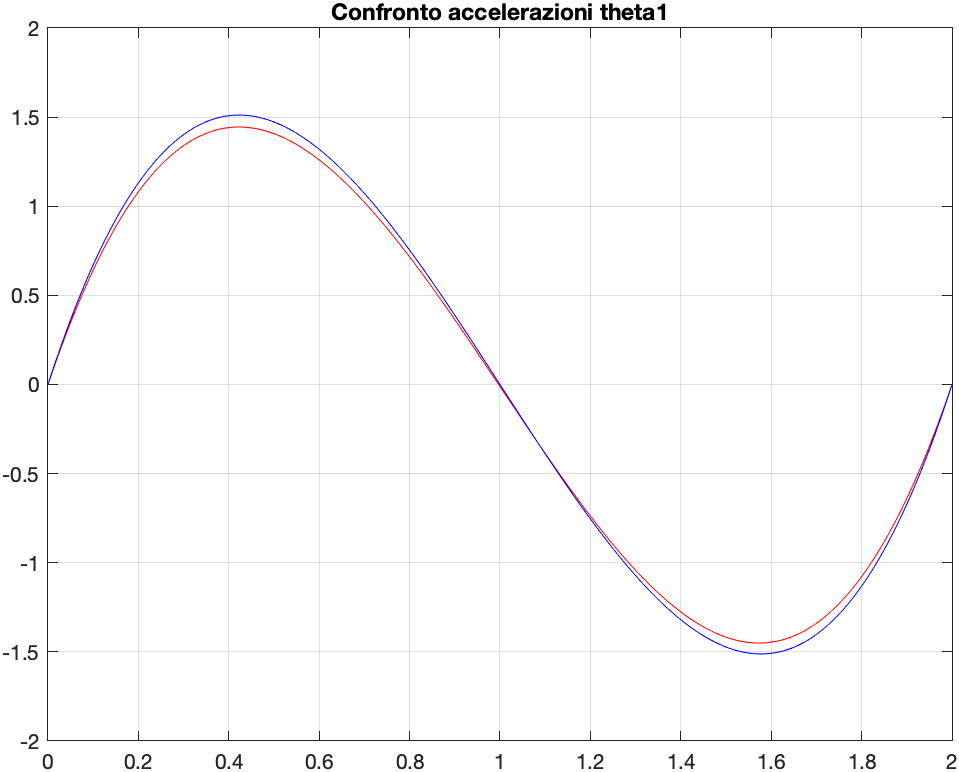
\includegraphics[width=.78\linewidth]{Immagini/Dinamica/confracct1.png}  
  \caption{Accelerazione $\theta_1$}
  \label{fig:sub-first}
\end{subfigure}
\begin{subfigure}{.45\textwidth}
  \centering
  % include second image
  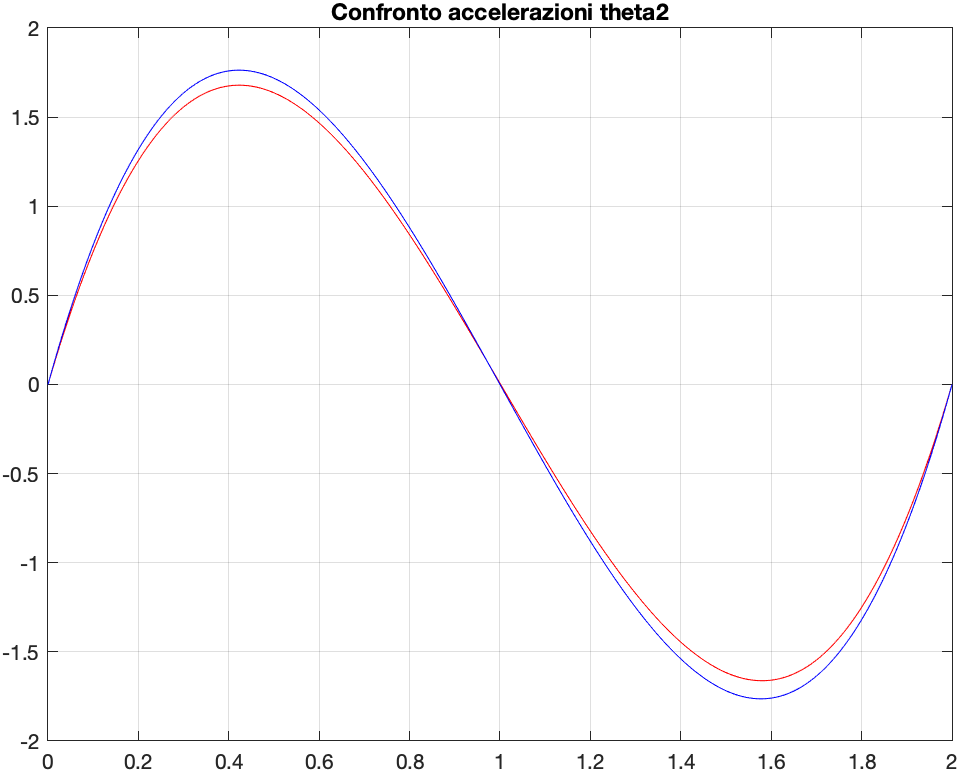
\includegraphics[width=.78\linewidth]{Immagini/Dinamica/confracct2.png}  
  \caption{Accelerazione $\theta_2$}
  \label{fig:sub-second}
\end{subfigure}
\caption{Confronto dinamica leggi di moto su accelerazioni}
\end{figure}
\begin{figure}[!ht]
\begin{subfigure}{.45\textwidth}
  \centering
  % include first image
  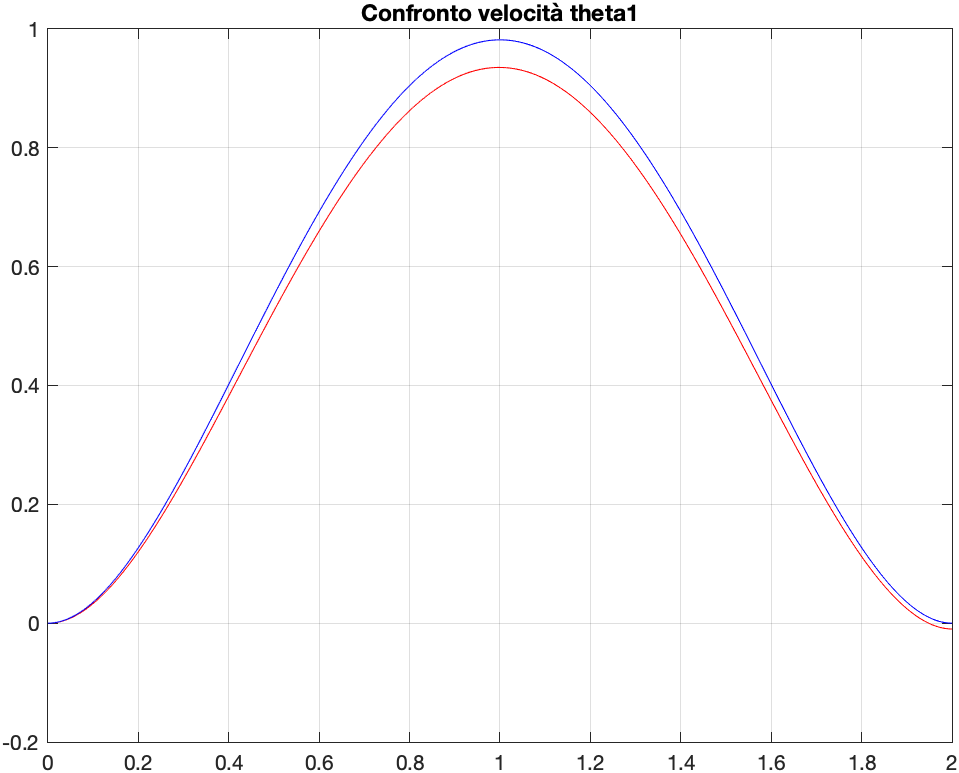
\includegraphics[width=.78\linewidth]{Immagini/Dinamica/confrvelt1.png}  
  \caption{Velocità $\theta_1$}
  \label{fig:sub-firstv}
\end{subfigure}
\begin{subfigure}{.45\textwidth}
  \centering
  % include second image
  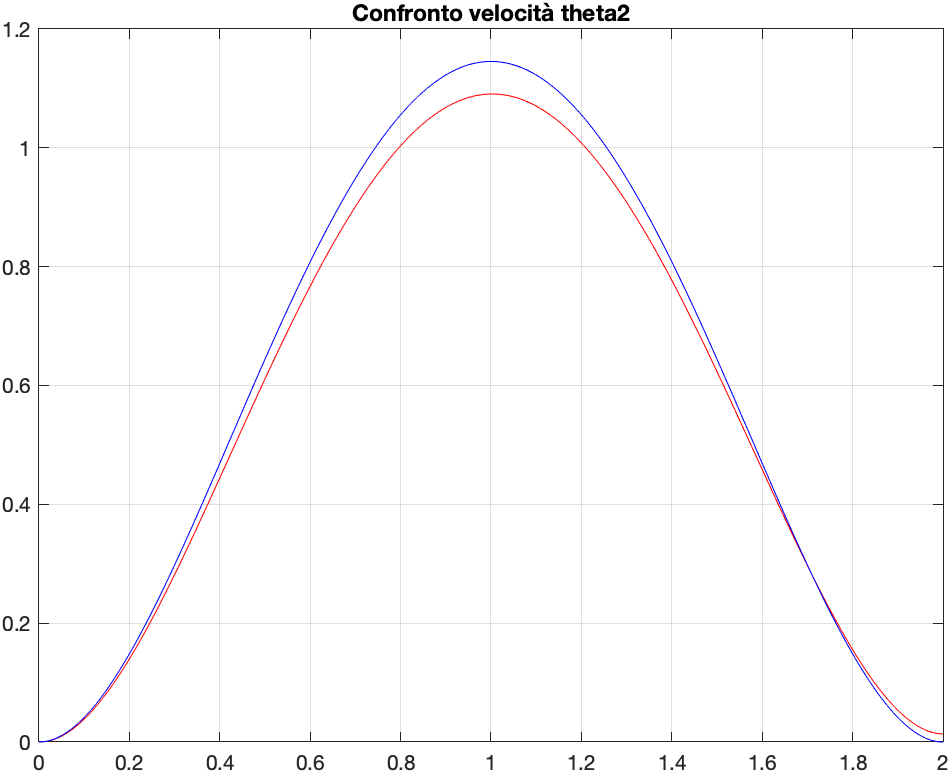
\includegraphics[width=.78\linewidth]{Immagini/Dinamica/confrtvelt2.png}  
  \caption{Velocità $\theta_2$}
  \label{fig:sub-secondv}
\end{subfigure}
\caption{Confronto dinamica leggi di moto su velocità}
\end{figure}
\begin{figure}[!ht]
\begin{subfigure}{.45\textwidth}
  \centering
  % include first image
  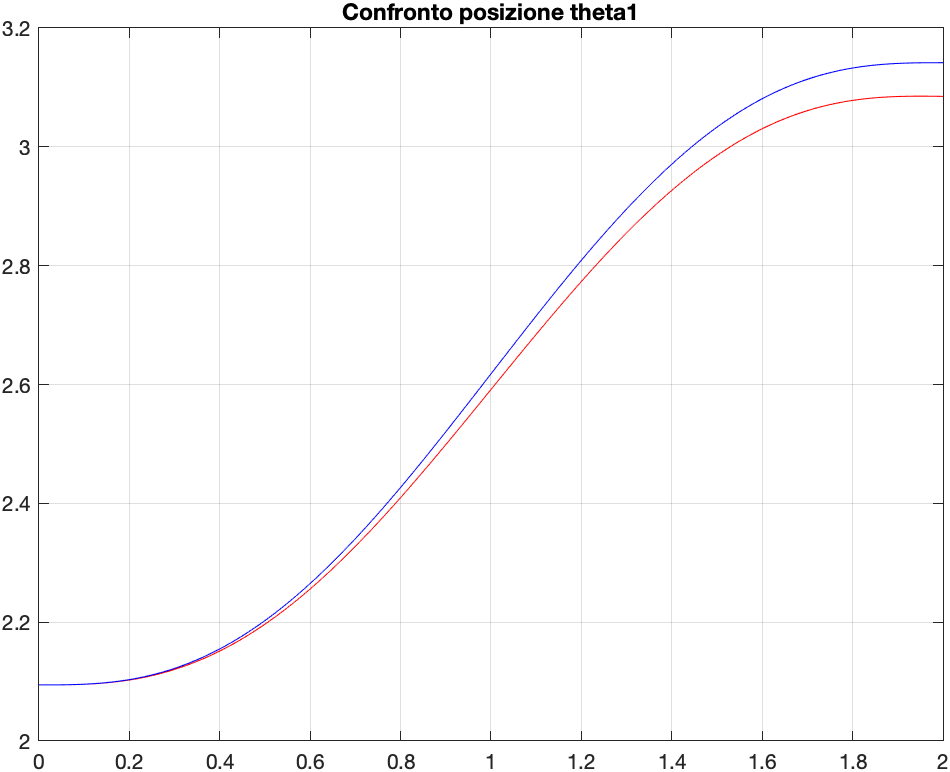
\includegraphics[width=.78\linewidth]{Immagini/Dinamica/confrpost1.png}  
  \caption{Posizione $\theta_1$}
  \label{fig:sub-firsta}
\end{subfigure}
\begin{subfigure}{.45\textwidth}
  \centering
  % include second image
  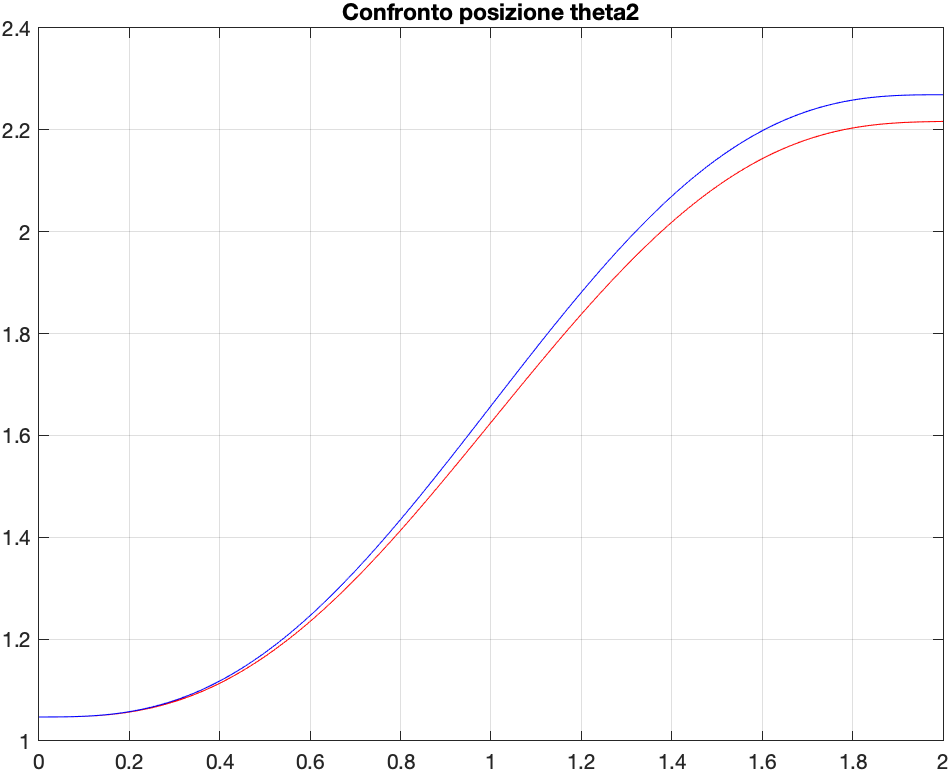
\includegraphics[width=.78\linewidth]{Immagini/Dinamica/confrpost2.png}  
  \caption{Posizione $\theta_2$}
  \label{fig:sub-seconda}
\end{subfigure}
\caption{Confronto dinamica leggi di moto su posizioni}
\end{figure}
\\Si può notare un errore tra le due curve dovuto al metodo di integrazione utilizzato.
\\Una volta calcolati tutti i parametri di nostro interesse andiamo a costruire il modello simulink che sarà utile per una visione d'insieme e per effettuare la validazione:
\begin{figure}[ht]
	\begin{center}
		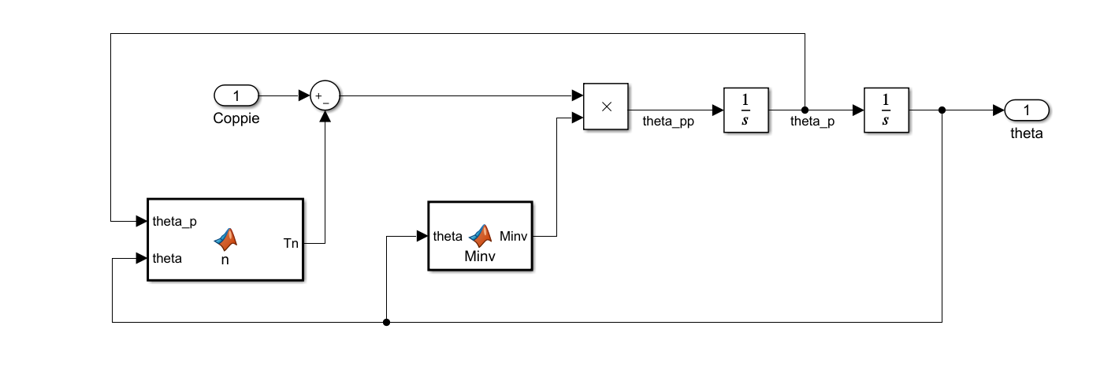
\includegraphics[scale=0.55]{Immagini/Dinamica/ModSimulink}
		\caption{Modello simulink manipolatore}
	\end{center}
\end{figure}
Il modello implementa l'equazione della dinamica diretta \ref{eq:dinamicaDiretta}, infatti riusciamo ad ottenere l'accelerazione a partire dalla moltiplicazione fra la matrice d'inerzia e la somma delle coppie con la matrice dei termini di Coriolis. Andando poi ad integrare otteniamo velocità e posizione che ci serviranno per trovare le accelerazioni negli step successivi.
\subsubsection*{Modellazione su Adams}
\addcontentsline{toc}{subsubsection}{Modellazione su Adams}
Per quanto riguarda la modellazione su Adams, è stato realizzato un prototipo dei link del manipolatore composto da aste rigide, i due link motorizzati sono fissati a terra mediante delle cerniere.
\begin{figure}[!ht]
	\begin{subfigure}{.5\textwidth}
		\centering
		% include first image
		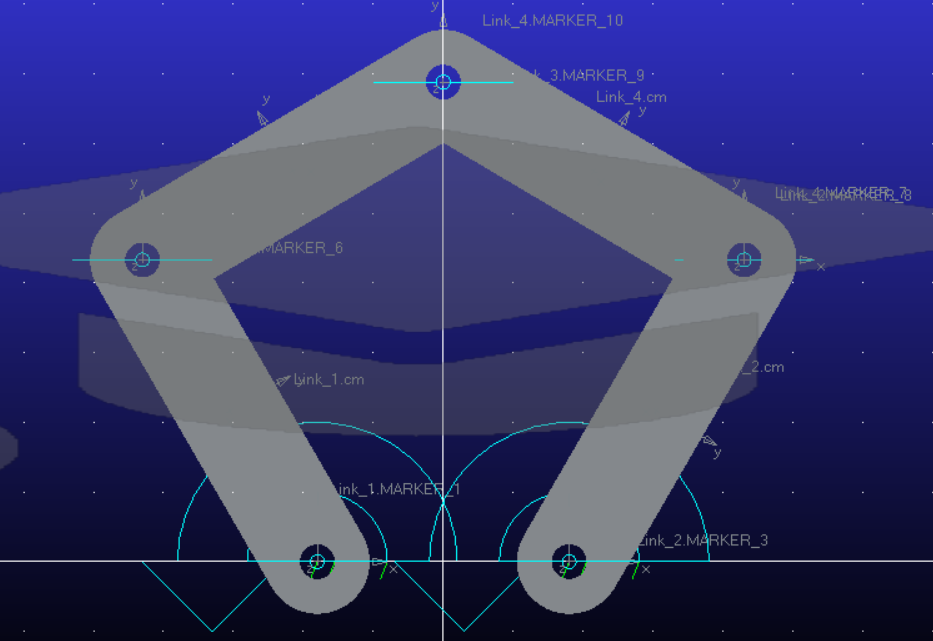
\includegraphics[width=.9\linewidth]{Immagini/Dinamica/adams1.png}  
		\caption{Vista dall'alto}
		\label{fig:sub-adams1}
	\end{subfigure}
	\begin{subfigure}{.5\textwidth}
		\centering
		% include second image
		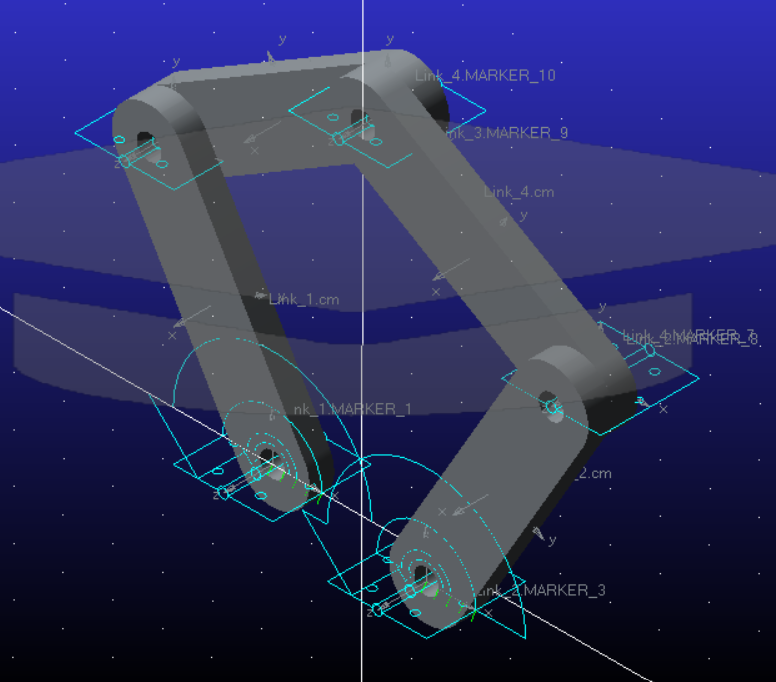
\includegraphics[width=.8\linewidth]{Immagini/Dinamica/adams2.png}  
		\caption{Vista in diagonale}
		\label{fig:sub-adams2}
	\end{subfigure}
	\caption{Modello Adams manipolatore 5R}
\end{figure}
Una volta definiti i vincoli e le modalità di movimento del manipolatore si è passati alla fase successiva ovvero quella dell'analisi del modello e della simulazione, andando ad assegnare le leggi di moto al modello Adams e verificando il suo comportamento rispetto al modello matlab.
\subsubsection*{Validazione e confronto}
\addcontentsline{toc}{subsubsection}{Validazione e confronto}
Le leggi di moto utilizzate per la validazione sono: 
\begin{table}[h!]
	\centering
	\begin{tabular}{|c|c|} 
		\hline
		Motore & Legge di moto  \\
		\hline\hline
		Motore 1 ($\theta_1$)& Sinusoidale $sin$ \\
		Motore 2 ($\theta_2$)& Sinusoidale $2\sin$ \\
		\hline
	\end{tabular}
	\caption{Leggi di moto validazione}
	\label{table:ldmAdams}
\end{table}
\\Una volta assegnata la legge ed eseguita la simulazione si è fatto un confronto:
\begin{figure}[!ht]
	\begin{subfigure}{.45\textwidth}
		\centering
		% include first image
		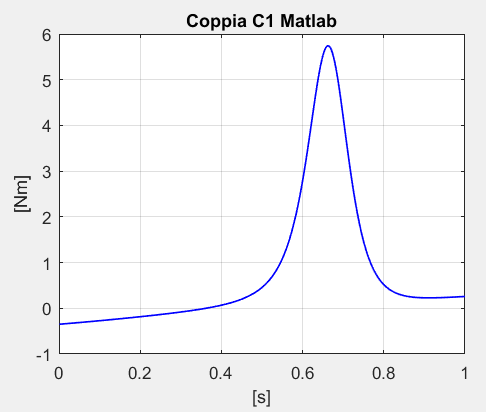
\includegraphics[width=.9\linewidth]{Immagini/Dinamica/c1matlab.png}  
		\caption{Coppia C1 Matlab}
		\label{fig:leggiC1M}
	\end{subfigure}
	\begin{subfigure}{.45\textwidth}
		\centering
		% include second image
		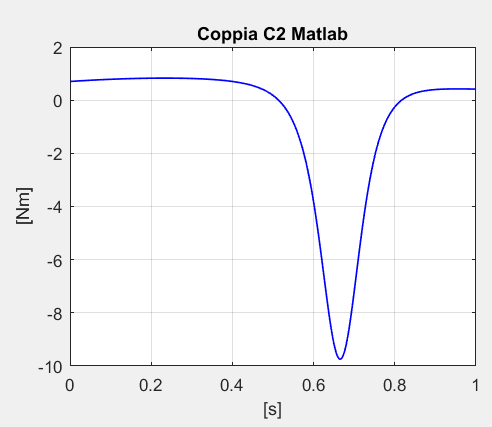
\includegraphics[width=.9\linewidth]{Immagini/Dinamica/c2matlab.png}  
		\caption{Coppia C2 Matlab}
		\label{fig:leggiC2M}
	\end{subfigure}
	\caption{Coppie in uscita Matlab}
\end{figure}
\begin{figure}[!ht]
	\begin{subfigure}{.45\textwidth}
		\centering
		% include first image
		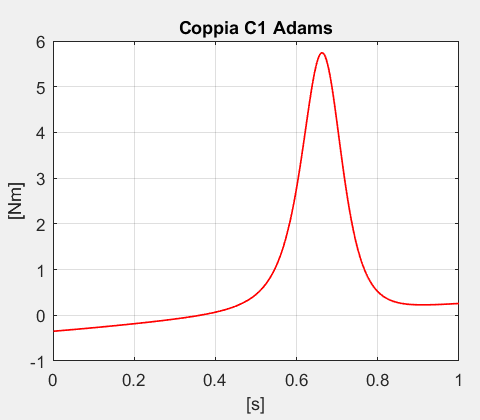
\includegraphics[width=.9\linewidth]{Immagini/Dinamica/c1adams.png}  
		\caption{Coppia C1 Adams}
		\label{fig:leggiC1A}
	\end{subfigure}
	\begin{subfigure}{.45\textwidth}
		\centering
		% include second image
		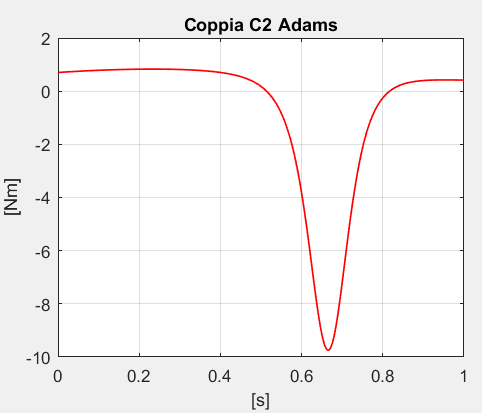
\includegraphics[width=.9\linewidth]{Immagini/Dinamica/c2adams.png}  
		\caption{Coppia C2 Adams}
		\label{fig:leggiC2A}
	\end{subfigure}
	\caption{Coppie in uscita Adams}
\end{figure}
\\Andando poi a fare una differenza tra questi due grafici riusciamo a trovare l'andamento dell'errore sulle coppie:
\begin{figure}[!ht]
	\begin{subfigure}{.5\textwidth}
		\centering
		% include first image
		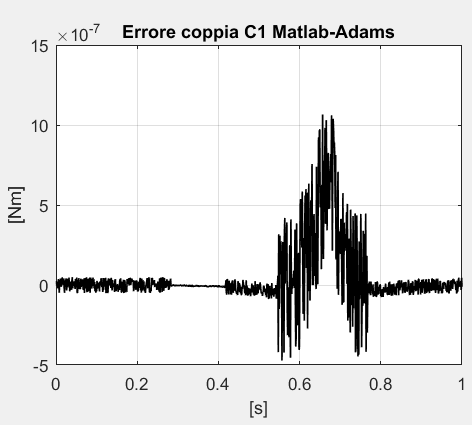
\includegraphics[width=.9\linewidth]{Immagini/Dinamica/confrc1.png}  
		\caption{Errore coppia C1}
		\label{fig:errC1}
	\end{subfigure}
	\begin{subfigure}{.5\textwidth}
		\centering
		% include second image
		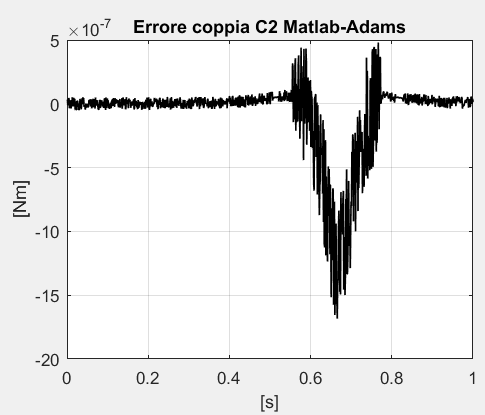
\includegraphics[width=.9\linewidth]{Immagini/Dinamica/confrc2.png}  
		\caption{Errore coppia C2}
		\label{fig:errC2}
	\end{subfigure}
	\caption{Errore Simulink-Adams}
\end{figure}
\\Analizzando il grafico vediamo che l'errore è nell'ordine di $10^{-7}$ di conseguenza è possibile vedere che la validazione ha portato un risultato positivo in quanto le coppie ottenute da matlab e quelle da Adams sono molto simili a parte un fattore d'errore dato dalle diverse modalità di calcolo due due software.
